\documentclass{thesisclass}
% Based on thesisclass.cls of Timo Rohrberg, 2009
% ----------------------------------------------------------------
% Thesis - Main document (Bachelor)
% ----------------------------------------------------------------

%\usepackage[ngerman]{babel}

%% -------------------------------
%% |  Information for PDF file   |
%% -------------------------------
\hypersetup{
 pdfauthor={Not set},
 pdftitle={Not set},
 pdfsubject={Not set},
 pdfkeywords={Not set}
}


%% ---------------------------------
%% | Information about the thesis  |
%% ---------------------------------

\newcommand{\myname}{Name}
\newcommand{\mytitle}{Title of thesis\\ 
											Second title line}
\newcommand{\myinstitute}{Institut f\"ur Experimentelle Kernphysik (IEKP)}
\newcommand{\mydepartment}{Fakult\"at f\"ur Physik}
\newcommand{\myuniversity}{Karlsruher Institut f\"ur Technologie}
\newcommand{\myplace}{Karlsruhe}


\newcommand{\reviewerone}{?}
\newcommand{\reviewertwo}{?}
%\newcommand{\advisor}{?}
%\newcommand{\advisortwo}{?}

\newcommand{\timestart}{XX. Monat 20XX}
\newcommand{\timeend}{XX. Monat 20XX}
\newcommand{\submissiontime}{DD. MM. 20XX}


%% ---------------------------------
%% | ToDo Marker - only for draft! |
%% ---------------------------------
% Remove this section for final version!
\setlength{\marginparwidth}{20mm}

\newcommand{\margtodo}
{\marginpar{\textbf{\textcolor{red}{ToDo}}}{}}

\newcommand{\todo}[1]
{{\textbf{\textcolor{red}{(\margtodo{}#1)}}}{}}


%% --------------------------------
%% | Old Marker - only for draft! |
%% --------------------------------
% Remove this section for final version!
\newenvironment{deprecated}
{\begin{color}{gray}}
{\end{color}}


%% --------------------------------
%% | Settings for word separation |
%% --------------------------------
% Help for separation:
% In german package the following hints are additionally available:
% "- = Additional separation
% "| = Suppress ligation and possible separation (e.g. Schaf"|fell)
% "~ = Hyphenation without separation (e.g. bergauf und "~ab)
% "= = Hyphenation with separation before and after
% "" = Separation without a hyphenation (e.g. und/""oder)

% Describe separation hints here:
\hyphenation{
% Pro-to-koll-in-stan-zen
% Ma-na-ge-ment  Netz-werk-ele-men-ten
% Netz-werk Netz-werk-re-ser-vie-rung
% Netz-werk-adap-ter Fein-ju-stier-ung
% Da-ten-strom-spe-zi-fi-ka-tion Pa-ket-rumpf
% Kon-troll-in-stanz
}


%% ------------------------
%% |    Including files   |
%% ------------------------
% Only files listed here will be included!
% Userful command for partially translating the document (for bug-fixing e.g.)
\includeonly{%
titlepage,
decleration,
introduction,
einleitung,
content,
beispielkapitel,
theorie,
evaluation,
conclusion,
zusammenfssung,
appendix
}


%%%%%%%%%%%%%%%%%%%%%%%%%%%%%%%%%
%% Here, main documents begins %%
%%%%%%%%%%%%%%%%%%%%%%%%%%%%%%%%%
\begin{document}

% Remove the following line for German text
%\selectlanguage{english}

\frontmatter
\pagenumbering{roman}
%% titlepage.tex
%%

% coordinates for the bg shape on the titlepage
\newcommand{\diameter}{20}
\newcommand{\xone}{-15}
\newcommand{\xtwo}{160}
\newcommand{\yone}{15}
\newcommand{\ytwo}{-253}

\begin{titlepage}
% bg shape
\begin{tikzpicture}[overlay]
\draw[color=gray]  
 		 (\xone mm, \yone mm)
  -- (\xtwo mm, \yone mm)
 arc (90:0:\diameter pt) 
  -- (\xtwo mm + \diameter pt , \ytwo mm) 
	-- (\xone mm + \diameter pt , \ytwo mm)
 arc (270:180:\diameter pt)
	-- (\xone mm, \yone mm);
\end{tikzpicture}
	\begin{textblock}{10}[0,0](4,2.5)
		
\includegraphics[width=.3\textwidth]{logos/KITLogo_RGB.pdf}
	\end{textblock}
        \begin{textblock}{11.9}[0,0](3.5,2.5)
          \changefont{phv}{m}{n}
          \raggedleft{\Large{IEKP-Bachelor-KA/201X-XX}}
        \end{textblock}
	\changefont{phv}{m}{n}	% helvetica	
	\vspace*{3.5cm}
	\begin{center}
		\Huge{\mytitle}
		\vspace*{1cm}\\
                \Large{\myname}
		\vspace*{2cm}\\
		\Large{
			\iflanguage{english}{Bachelor Thesis}			
												  {Bachelorarbeit}
		}\\
		\vspace*{1cm}
		\huge{\myname}\\
		\vspace*{1cm}
		\Large{
			\iflanguage{english}{At the Department of Physics}			
													{An der Fakult\"at f\"ur Physik}
			\\
			\myinstitute
		}
	\end{center}
	\vspace*{1cm}
\Large{
\begin{center}
\begin{tabular}[ht]{l c l}
  % Gutachter sind die Professoren, die die Arbeit bewerten. 
  \iflanguage{english}{Reviewer}{Erstgutachter}: & \hfill  & \reviewerone\\
  \iflanguage{english}{Second reviewer}{Zweitgutachter}: & \hfill  & \reviewertwo%\\
  %\iflanguage{english}{Advisor}{Betreuender Mitarbeiter}: & \hfill  & \advisor\\
  %\iflanguage{english}{Second advisor}{Zweiter betreuender Mitarbeiter}: & \hfill  & \advisortwo\\
  % Der zweite betreuende Mitarbeiter kann weggelassen werden. 
\end{tabular}
\end{center}
}


\vspace{2cm}
\begin{center}
%\large{\iflanguage{english}{Duration:}{Bearbeitungszeit}: \timestart
%\hspace*{0.25cm} -- \hspace*{0.25cm} \timeend}
\large{\myplace, \timeend}
\end{center}


\begin{textblock}{10}[0,0](4,16.8)
\tiny{ 
	\iflanguage{english}
		{KIT -- University of the State of Baden-Wuerttemberg and National Research Center of the Helmholtz Association}
		{KIT -- Universit\"at des Landes Baden-W\"urttemberg und nationales Forschungszentrum in der Helmholtz-Gemeinschaft}
}
\end{textblock}

\begin{textblock}{10}[0,0](14,16.75)
\large{
	\textbf{www.kit.edu} 
}
\end{textblock}

\end{titlepage}

\vspace*{36\baselineskip}
\hbox to \textwidth{\hrulefill}
\par
\iflanguage{english}{I declare that I have developed and written the enclosed thesis completely by myself, and have not used sources or means without declaration in the text.}{Ich versichere wahrheitsgem\"a\ss, die Arbeit selbstst\"andig angefertigt, alle benutzten Hilfsmittel vollst\"andig und genau angegeben und alles kenntlich gemacht zu haben, was aus Arbeiten anderer unver\"andert oder mit Ab\"anderungen entnommen wurde.}

\textbf{PLACE, DATE}
\vspace{1.5cm}

\dotfill\hspace*{8.0cm}\\
\hspace*{2cm}(\textbf{YOUR NAME}) %center name with hspace

\thispagestyle{empty}
\blankpage


%% -------------------
%% |   Directories   |
%% -------------------
\tableofcontents
\blankpage


%% -----------------
%% |   Main part   |
%% -----------------
\mainmatter
\pagenumbering{arabic}
%% einleitung.tex
%%

%% ==============================
\chapter{Einleitung}
\label{ch:Einleitung}
%% ==============================

{\bibliographystyle{babunsrt-fl}}

Bei der Untersuchung der Teilchenkollisionen im Large-Hadron-Collider am CERN werden von den Detektoren gewaltige Datenmengen aufgezeichnet. Um diese Datenmengen effizient auszuwerten, ist die Anwendung von multivariaten Datenanalysemethoden n\"otig.

Multivariate Analysealgorithmen sind in vielen Bereichen der Teilchenphysik unumg\"anglich. Eine Anwendung ist die Klassifikation von Ereignissen in Untergr\"unde und gesuchtes Signal. Besonders wichtig ist dies unter anderem bei der Suche nach Higgs-Boson-Produktion in Assoziation mit einem Top-Quark-Antiquark-Paar (\ttH), da bei diesem Prozess aufgrund der Vorhersage des Standardmodells nur wenige Signalereignisse zu erwarten sind. Um Analysen wie diese m\"oglichst effizient zu gestalten, ist es wichtig m\"oglichst gute Algorithmen zu nutzen.

Multivariate Analysemethoden spielen jedoch nicht nur in der Physik eine wichtige Rolle, sondern sind auch bei Problematiken wie der Sprach- oder Schrifterkennung oder Bewertungen des Aktienmarktes einsetzbar. Durch diese Vielzahl von Anwendungsgebieten entstehen viele verschiedene Implementierungen unterschiedlicher Algorithmen. Insbesondere das Interesse der freien Wirtschaft f\"ordert die Weiterentwicklung und Erforschung multivariater Methoden.

In einer Studie vergleicht J. Wainer \cite{DBLP:journals/corr/Wainer16} beispielsweise verschiedene Klassifikations-Algorithmen. Dazu wendet er die Algorithmen auf verschiedene \"offentlicher Datens\"atze an und variiert die Parameter der Klassifikatoren. Allerdings ist dieser Vergleich ziemlich allgemein gehalten und setzt kein klares Anwendungsgebiet f\"ur die Algorithmen voraus.

Um eine m\"ogliche Anwendung in der Teilchenphysik zu pr\"ufen, ist es von Interesse verschiedene Algorithmen im Kontext einer physikalischen Analyse zu untersuchen.

In dieser Arbeit werden drei verschiedene Implementationen des Gradient-Boosting-\\Algorithmus anhand der Nutzung zur \ttH-Analyse getestet und verglichen. Dazu sind in Kapitel \ref{ch:Theorie} zun\"achst die wichtigsten theoretischen Grundlagen \"uber das Standardmodell der Teilchenphysik und die \ttH-Produktion zusammengefasst. Darauf folgt in Kapitel \ref{ch:experiment} ein kurzer \"Uberblick \"uber das CMS-Experiment und die \ttH-Analyse. Kapitel \ref{ch:algorithmen} handelt von multivariater Datenanalyse im Allgemeinen und Boosted Decision Trees im Speziellen. Der Vergleich der Algorithmen wird in Kapitel \ref{ch:vergleich} beschrieben. Abschlie\ss end folgt in Kapitel \ref{ch:Fazit} ein Fazit mit einem kurzen Ausblick \"uber zuk\"unftig m\"ogliche Entwicklungen.
%% beispielkapitel.tex
%%

%% ==============
\chapter{Kapitel 1}
\label{ch:Kapitel1}
%% ==============

Der Titel der Kapitel sollte entsprechend angepasst werden, z.B. 
Kpitel 1 nach 'Das CMS Experiment' und entsprechend die Abschnitte 
umbenannt werden z.B. 'Der Silizumstreifen Detektor' oder 'Der Pixel 
Detektor'.  

Es ist eine gute Idee ein eigenes File f\"ur jedes Kapitel anzulegen.

%% ===========================
\section{Einbinden von Grafiken}
\label{ch:Kapitel1:sec:Grafiken}
%% ===========================

Grafiken werden mit 'inlcudegrapghics' eigebunden, f\"ur hier
benutzte Vorlage sollten 'pdf' Grafiken eingebunden werden.  

\begin{verbatim}
\begin{figure}[hhh]
 \begin{center}
   
\includegraphics[width=.3\textwidth]{logos/KITLogo_RGB.pdf}
   \parbox[b]{12cm}{
     \caption[Beispiel Abbildung (kurze Unterschrift f\"ur Abbildungsverzeichnis)]
             {\label{fig:exmaple} \it Beispiel Abbildung
               (ausf\"uhrliche Bildunterschrift, die unter dem Bild
               angezeigt wird)}
   }
 \end{center}
\end{figure}
\end{verbatim}

\begin{figure}[hhh]
 \begin{center}
   
\includegraphics[width=.3\textwidth]{logos/KITLogo_RGB.pdf}
   \parbox[b]{12cm}{
     \caption[Beispiel Abbildung (kurze Unterschrift f\"ur Abbildungsverzeichnis)]
             {\label{fig:exmaple} \it Beispiel Abbildung
               (ausf\"uhrliche Bildunterschrift, die unter dem Bild
               angezeigt wird)}
   }
 \end{center}
\end{figure}




\dots


%% ===========================
\section{Ertellen von Tabellen}
\label{ch:Kapitel1:sec:Tabellen}
%% ===========================

\begin{verbatim}
\begin{table}[hhh]\parbox{12cm}{
  \caption[Physical constants]
  {\it Beisspiel: Tabelle physikalischer  Konstanten{\rm \cite{Beringer:1900zz}}
  }\label{tab:physconst}}
  \begin{tabular}{lll}
  \hline
  {\bf Symbol} & {\bf Beschreibung} & {\bf Einheit}  \\
  \hline \hline
     $c$    & Lichtgeschwindigkeit  &  $299792458$~ms$^{-1}$ \\
     $h$    & Planck Konstante & $6.626098 \times 10^{-34}$~Js \\
     $\hbar = \frac{h}{2 \pi}$ & Planck Konstante, reduziert &
            $1.054571 \times 10^{-34}$~Js \\
     $e$    & elektrische Elementarladung & $1.602176 \times 10^{-19}~C$ \\ 
  $\epsilon_0$ & elektrische Feldkontante & 
                  $8.854187 \times 10^{-12}$~Fm$^{-1}$ \\
  $\mu_0$       & magnetische Feldkonstante & $4\pi \times 
          10^{-7}$~NA$^{-2} = 12.566270 \times 10^{-7}$~NA$^{-2}$ \\
   $m_e$  & Elektronen Masse             &  $0.510998$~MeV/c$^2$\\
   $m_p$  & Protonen Masse               &  $938.271998$~MeV/c$^2$ \\        
   $N_A$  & Avogadro Zahl         & $6.022144 \cdot 
                                        10^{23}~{\rm mol}^-1 $ \\
   $r_e$  & Elektronenradius & $2.817940 \cdot 10^{-13}$~cm \\                                     
  \hline
  \end{tabular}
\end{table}
\end{verbatim}

\begin{table}[hhh]\parbox{12cm}{
  \caption[Physical constants]{\it Beisspiel: Tabelle physikalischer  Konstanten{\rm \cite{Beringer:1900zz}}
  }\label{tab:physconst}}
  \begin{tabular}{lll}
  \hline
  {\bf Symbol} & {\bf Beschreibung} & {\bf Einheit}  \\
  \hline \hline
     $c$    & Lichtgeschwindigkeit  &  $299792458$~ms$^{-1}$ \\
     $h$    & Planck Konstante & $6.626098 \times 10^{-34}$~Js \\
     $\hbar = \frac{h}{2 \pi}$ & Planck Konstante, reduziert &
            $1.054571 \times 10^{-34}$~Js \\
     $e$    & elektrische Elementarladung & $1.602176 \times 10^{-19}~C$ \\ 
  $\epsilon_0$ & elektrische Feldkontante & 
                  $8.854187 \times 10^{-12}$~Fm$^{-1}$ \\
  $\mu_0$       & magnetische Feldkonstante & $4\pi \times 
          10^{-7}$~NA$^{-2} = 12.566270 \times 10^{-7}$~NA$^{-2}$ \\
   $m_e$  & Elektronen Masse             &  $0.510998$~MeV/c$^2$\\
   $m_p$  & Protonen Masse               &  $938.271998$~MeV/c$^2$ \\        
   $N_A$  & Avogadro Zahl         & $6.022144 \cdot 
                                        10^{23}~{\rm mol}^-1 $ \\
   $r_e$  & Elektronenradius & $2.817940 \cdot 10^{-13}$~cm \\                                     
  \hline
  \end{tabular}
\end{table}



\dots


%% ===========================
\section{Benutzung n\"utzlicher Pakete}
\label{ch:Kapitel1:sec:Pakete}
%% ===========================

%% ===========================
\subsection{SI Einheiten: siunitx}
\label{ch:Kapitel1:subsec:SiUnit}
%% ===========================

Das Paket siunitx bietet die M\"oglichkeit Einheiten und Zahlen
schnell und einfach darzustellen.\\
Beispiel Code:
\begin{verbatim}
\si{kg.m.s^{-1}} \\
\si{\kilogram\metre\per\second} \\
\si[per-mode=symbol]{\kilogram\metre\per\second} \\
\si[per-mode=symbol]{\kilogram\metre\per\ampere\per\second}
\end{verbatim}
Ausgabe im Text''\\
\si{kg.m.s^{-1}} \\
\si{\kilogram\metre\per\second} \\
\si[per-mode=symbol]{\kilogram\metre\per\second} \\
\si[per-mode=symbol]{\kilogram\metre\per\ampere\per\second}


Eine Einf\"uhrung in das Paket findet man unter:
\begin{verbatim}
ftp://ftp.dante.de/tex-archive/macros/latex/exptl/siunitx/siunitx.pdf
\end{verbatim}

%% ===========================
\subsection{amsmath}
\label{ch:Kapitel1:subsec:amsmath}
%% ===========================

\begin{verbatim}
ftp://ftp.ams.org/pub/tex/doc/amsmath/short-math-guide.pdf
\end{verbatim}

%% ===========================
\subsection{xxx}
\label{ch:Kapitel1:subsec:xxx}
%% ===========================
%% Theorie.tex
%%
%\usepackage[ngerman]{babel}
%% ==============
\chapter{Theoretische Grundlagen}
\label{ch:Theorie}
%% ==============

{\bibliographystyle{babalpha-fl}}	% german style

Das Standardmodell der Teilchenphysik beschreibt die bisher bekannten Bausteine der Materie sowie deren Wechselwirkungen. In Kapitel \ref{ch:Theorie:sec:Standardmodell} wird ein kurzer \"Uberblickblick dar\"uber gegeben, woraufhin in Abschnitt \ref{ch:Theorie:sec:ttH} genauer auf die Produktion von Higgs-Bosonen und Topquarks eingegangen wird.\\


%% ===========================
\section{Das Standardmodell der Teilchenphysik}
\label{ch:Theorie:sec:Standardmodell}
%% ===========================

Der folgende Abschnitt soll einen kurzen \"Uberblick \"uber das Standardmodell der Elementarteilchenphysik geben, dabei bezieht er sich meist auf \cite{SWB-39819646X}.

Das Standardmodell der Elementarteilchenphysik ist eine Quantenfeldtheorie, die die Theorie der elektroschwachen Wechselwirkung mit der Quantenchromodynamik zusammenfasst und vereinheitlicht. Das Universum besteht aus einigen grundlegenden Bausteinen, die durch vier elementare Kr\"afte beeinflusst werden \cite{O'Luanaigh:1997201}. Die bislang beste Beschreibung dieses Aufbaus liefert das Standardmodell, wenngleich es die vierte Kraft, die Gravitation, nicht erkl\"aren kann. Dennoch war es mit diesem Modell m\"oglich fast alle experimentellen Ergebnisse zu best\"atigen, sowie sehr pr\"azise Vorhersagen \"uber verschiedene Ph\"anomene zu treffen.

Die bislang entdeckte Materie besteht aus zwei Arten von Elementarteilchen, den Leptonen sowie den Quarks. Diese lassen sich jeweils in drei Familien unterteilen. Jede Quark-Familie besteht jeweils aus einem Quarkpaar und deren Antiteilchen, diese sind Up- und Down-, Strange- und Charm- sowie Bottom- und Topquark.\\
Leptonen bilden jeweils zusammen mit dem dazugeh\"origen Neutrino und den jeweiligen Antiteilchen eine Familie. Im Gegensatz zu den Quarks unterliegen Leptonen nicht der starken Wechselwirkung.\\
Die dritte elementare Wechselwirkung, die im Standardmodell beschrieben ist, ist die elektromagnetische Wechselwirkung. Ihr unterliegen alle geladenen Teilchen. Diese Wechselwirkungen sind in ihrer Struktur sehr \"ahnlich und werden durch den Austausch von Vektorbosonen vermittelt. Diese sind die Gluonen der starken Wechselwirkung, die W- und Z-Bosonen der schwachen Wechselwirkung und die Photonen ($\gamma$) der elektromagnetischen. W\"ahrend die Fermionen aus denen die Materie besteht, einen halbzahligen Spin besitzen, haben die Bosonen einen ganzzahligen Spin.

Der letzte fehlende Baustein im Standardmodell ist ein elementares Spin-0 Teilchen, ohne das keine konsistente Erkl\"arung f\"ur die W und Z$^0$ Massen m\"oglich w\"are. Dieses ist das Higgs-Boson, welches 2012 am CERN entdeckt wurde. Die Kopplung zwischen Higgs-Boson und anderen Elementarteilchen ist proportional zur Fermionenmasse. In Abbildung \ref{fig:Standardmodell} sind alle elementaren Bosonen und Fermionen dargestellt.

\begin{figure}[hhh]
 \begin{center}
   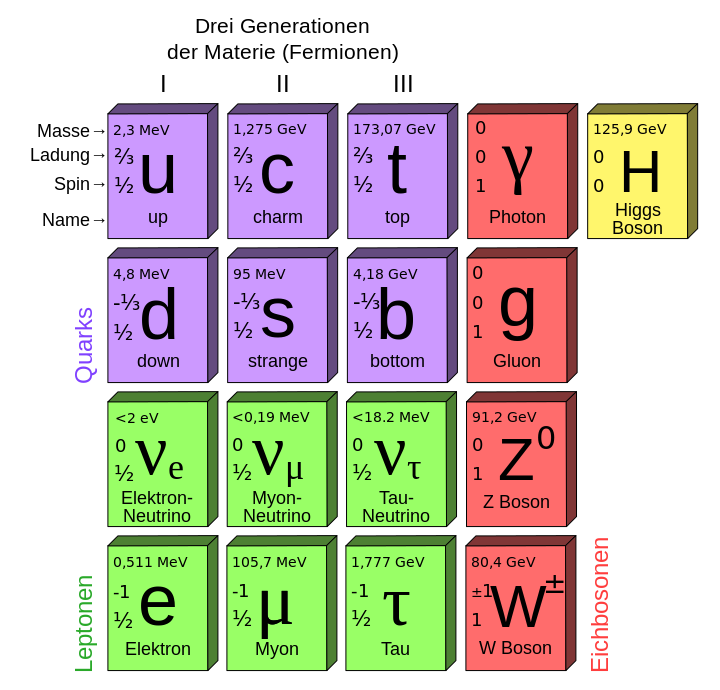
\includegraphics[width=\textwidth]{graphics/Standard_Model.png}
   \parbox[b]{12cm}{
     \caption[Standardmodell der Teilchenphysik]
             {\label{fig:Standardmodell} \it\!Die 12 fundamentalen Fermionen und 5 fundamentalen Bosonen des Standardmodells der Teilchenphysik,\\ Quelle: \cite{wiki:Standardmodell}}
   }
 \end{center}
\end{figure}

Insgesamt stimmen die experimentellen Ergebnisse gut mit den Vorhersagen des Standardmodells \"uberein. Dennoch reicht das Modell nicht aus, um s\"amtliche Ph\"anomene zu erkl\"aren. Im Modell werden beispielsweise masselose Neutrinos gefordert, allerdings wird zur Erkl\"arung der beobachteten Neutrinooszillationen die Existenz massiver Neutrinos ben\"otigt.

%% ===========================
\section{Assoziierte Higgs-Boson-Top-Quark-Paar-Produktion (\ttH)}
\label{ch:Theorie:sec:ttH}
%% ===========================

Da die Kopplungskonstante des Higgs-Mechanismus im Standardmodell von der Fermionenmasse abh\"angt, ist eine Untersuchung der Kopplung zwischen Top-Quark und Higgs-Boson aufgrund der hohen Masse des Top-Quarks verglichen mit anderen Quarkmassen, besonders interessant. In Tabelle \ref{tab:quarkmasse} sind zum Vergleich die Quarkmassen aufgelistet.\\


\begin{table}[hhh]\parbox{12cm}{
  \caption[Quarkmassen]{\it\!Tabelle mit Quarkmassen {\rm \cite{Agashe:2014kda}}
  }\label{tab:quarkmasse}}
  \begin{center}
  \begin{tabular}{lll}
  \hline
  {\bf Quark} & {\bf Symbol} & {\bf Masse}  \\
  \hline \hline
     Up		& u & $\num{2,3}^{{+0,7}}_{{-0,5}}\si{\mega\electronvolt}$ \\
     Down	& d & $\num{4,8}^{{+0,5}}_{{-0,3}}\si{\mega\electronvolt}$ \\
     Strange& s & $\num{95}\pm \num{5}\si{\mega\electronvolt}$ \\
     Charm	& c & $\num{1,275}\pm \num{0,025}\si{\giga\electronvolt}$ \\ 
  	 Bottom & b & $\num{4,18}\pm \num{0,03}\si{\giga\electronvolt}$ \\
     Top    & t & $\num{173,07}\pm \num{0,52}\pm \num{0,72}\si{\giga\electronvolt}$ \\                                   
  \hline
  \end{tabular}
  \end{center}
\end{table}

Diese Kopplung kann w\"ahrend der assoziierten Produktion eines Higgs-Bosons mit einem Paar aus Top-Quark und Anti-Top-Quark untersucht werden.\\
Wechselwirkungen zwischen Teilchen k\"onnen durch Feynman-Diagramme visualisiert werden. In Abbildung \ref{fig:ttH_feynmans} sind exemplarisch einige Feynmandiagramme zur \ttH-Produktion in f\"uhrender Ordnung abgebildet und zum Vergleich das Feynmandiagramm der Gluon-Gluon-Fusion, dem dominierenden Kanal der Higgs-Boson-Produktion am LHC, in Abbildung \ref{fig:gluonfusion}.

\begin{figure}[hhh]
 \begin{center}
   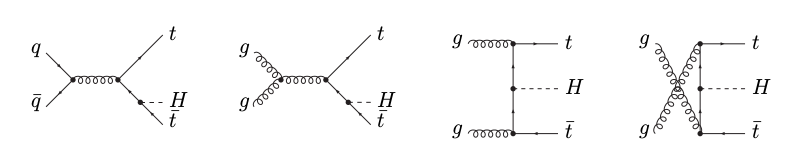
\includegraphics[width=\textwidth]{graphics/ttH_feynmans.png}
   \parbox[b]{12cm}{
     \caption[\ttH Feynman-Diagramme]
             {\label{fig:ttH_feynmans} \it\!Feynman-Diagramme f\"ur die \ttH-Produktion aus Hadronenkollisionen in f\"uhrender Ordnung \cite{hep-ph/0211352}}
   }
 \end{center}
\end{figure}

\begin{figure}[hhh]
 \begin{center}
   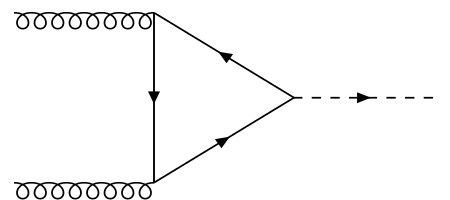
\includegraphics[width=0.4\textwidth]{graphics/gluonfusion.png}
   \parbox[b]{12cm}{
     \caption[Gluon-Gluon-Fusion Feynman-Diagramm]
             {\label{fig:gluonfusion} \it\!Feynman-Diagramm f\"ur die Gluon-Gluon-Fusion, dem dominierenden Kanal der Higgs-Boson-Produktion am LHC, erstellt mit \cite{feynman_draw}}
   }
 \end{center}
\end{figure}
%% zusammenfassung.tex
%%

%% ==================
\chapter{Fazit und Ausblick}
\label{ch:Fazit}
%% ==================

{\bibliographystyle{babunsrt-fl}}

In diesem Kapitel sollen nochmals alle Resultate zusammengefasst und ein Fazit gezogen werden. Anschlie\ss end wird ein kurzer Ausblick gegeben.

Insgesamt sind in der Kategorie mit mindestens sechs Jets und mindestens vier B-Tags keine signifikanten Unterschiede in den ROC-Kurven und somit in der G\"ute der getesteten Algorithmen zu erkennen. In der Kategorie mit mindestens sechs Jets und zwei B-Tags, die sehr viele Untergrundereignisse und nur wenig Signalereignisse aufweist, ist der TMVA-Algorithmus etwas schlechter als der in Scikit-Learn implementierte und XGBoost. Die Unterschiede sind allerdings nicht signifikant genug, als dass ein Wechsel zu einem der anderen Algorithmen unbedingt n\"otig w\"are.

W\"ahrend der Untersuchungen mit den verschiedenen BDTs stellte sich heraus, dass die besten Ergebnisse, unabh\"angig vom verwendeten Algorithmus, bei einer gro\ss en Anzahl Entscheidungsb\"aumen (etwa 2000) und kleiner Lernrate ($\leq \num{0,01}$) erzielt werden. Und auch wenn sich zwischen einzelnen Algorithmen kaum signifikante Unterschiede ergeben, lohnt es sich, geeignete Parameter zu suchen. Mit gut gew\"ahlten Parametern l\"asst sich die Klassifikation jedes Algorithmus verbessern. Allerdings wird es immer M\"oglichkeiten geben die Einstellungen so zu ver\"andern, dass sich die Klassifikation etwas verbessert. Es gilt abzuw\"agen inwieweit eine marginale Verbesserung die deutlich l\"angeren Trainingszeiten rechtfertigt.\\
Ein weiteres Mittel die Klassifikation der BDTs zu verbessern, ist die Wahl geeigneter Eingangsvariablen, auf die in dieser Arbeit nicht eingegangen wurde. Somit kann auch ohne gro\ss e Unterschiede zwischen verschiedenen Algorithmen eine Verbesserung der Optionen einzelner BDT-Implementierungen wertvoll f\"ur die \ttH-Analyse sein.

Auf jeden Fall sollte weiterhin getestet werden, ob es Klassifikatoren gibt, die bessere Ergebnisse erzielen. Es w\"are beispielsweise auch interessant komplett andere Klassifikatoren wie Random Forests oder Neuronale Netze zu testen.

Der n\"achste Schritt sollte sein, weitere multivariate Algorithmen neben TMVA in das CMSSW-Framework zu integrieren, um weitere Tests zu vereinfachen.


%% --------------------
%% |   Bibliography   |
%% --------------------
\cleardoublepage
\phantomsection
\addcontentsline{toc}{chapter}{\bibname}

\iflanguage{english}
{\bibliographystyle{IEEEtranSA}}	% english style
{\bibliographystyle{babalpha-fl}}	% german style
												  
% Use IEEEtran for numeric references
%\bibliographystyle{IEEEtranSA})

\bibliography{thesis}


%% ----------------
%% |   Appendix   |
%% ----------------
\cleardoublepage

%% appendix.tex
%%

%% ==============================
%\chapter{Appendix}
%\label{ch:Appendix}
%% ==============================

\appendix

\iflanguage{english}
{\addchap{Appendix}}	% english style
{\addchap{Anhang}}	% german style


%\iflanguage{english}
%{\section{First Appendix Section}
%		\label{Anhang-Implementierung}}
%{\section{Anhang}
%		\label{Anhang-Implementierung}}


\begin{table}[hhh]\parbox{12cm}{
\renewcommand\thetable{A.1}
  \caption[Scikit-Learn 6j4t Ergebnisse]{Tabelle mit Trainingsresultaten des Scikit-Learn-Algorithmus f\"ur verschiedene Parametereinstellungen in der 6-Jet-4-B-Tag-Kategorie}% {\rm \cite{Agashe:2014kda}}
  }\label{tab:sklearn_6j4t}
  \begin{center}
  \begin{tabular}{lllll}
  \hline
  learning\_rate & n\_estimators & ROC-Integral & P(KS) Signal & P(KS) Untergrund\\
  \hline
\num{0,001}  & \num{1500} & \num{0,729} & \num{0,13} & \num{0,59}\\
\num{0,0028} & \num{1500} & \num{0,732} & \num{0,27} & \num{0,83}\\
\num{0,0046} & \num{1500} & \num{0,733} & \num{0,31} & \num{0,75}\\
\num{0,0064} & \num{1500} & \num{0,733} & \num{0,21} & \num{0,82}\\
\num{0,0082} & \num{1500} & \num{0,734} & \num{0,08} & \num{0,77}\\
\num{0,001}  & \num{1700} & \num{0,73}  & \num{0,11} & \num{0,6}\\
\num{0,0028} & \num{1700} & \num{0,732} & \num{0,24} & \num{0,82}\\
\num{0,0046} & \num{1700} & \num{0,733} & \num{0,34} & \num{0,78}\\
\num{0,0064} & \num{1700} & \num{0,734} & \num{0,14} & \num{0,77}\\
\num{0,0082} & \num{1700} & \num{0,734} & \num{0,04} & \num{0,7}\\
\num{0,001}  & \num{1900} & \num{0,73}  & \num{0,09} & \num{0,74}\\
\num{0,0028} & \num{1900} & \num{0,732} & \num{0,25} & \num{0,85}\\
\num{0,0046} & \num{1900} & \num{0,733} & \num{0,23} & \num{0,85}\\
\num{0,0064} & \num{1900} & \num{0,734} & \num{0,08} & \num{0,72}\\
\num{0,0082} & \num{1900} & \num{0,734} & \num{0,03} & \num{0,67}\\
\num{0,001}  & \num{2100} & \num{0,730} & \num{0,13} & \num{0,77}\\
\num{0,0028} & \num{2100} & \num{0,733} & \num{0,27} & \num{0,81}\\
\num{0,0046} & \num{2100} & \num{0,733} & \num{0,19} & \num{0,83}\\
\num{0,0064} & \num{2100} & \num{0,734} & \num{0,04} & \num{0,69}\\
\num{0,0082} & \num{2100} & \num{0,734} & \num{0,02} & \num{0,6}\\
\num{0,001}  & \num{2300} & \num{0,730} & \num{0,17} & \num{0,81}\\
\num{0,0028} & \num{2300} & \num{0,733} & \num{0,32} & \num{0,81}\\
\num{0,0046} & \num{2300} & \num{0,734} & \num{0,14} & \num{0,8}\\
\num{0,0064} & \num{2300} & \num{0,734} & \num{0,02} & \num{0,66}\\
\num{0,0082} & \num{2300} & \num{0,734} & \num{0,01} & \num{0,45}\\
  \hline
  \end{tabular}
  \end{center}
\end{table}

\begin{table}[tbp]\parbox{12cm}{
\renewcommand\thetable{A.2}
  \caption[XGBoost 6j4t Ergebnisse]{Tabelle mit Trainingsresultaten des XGBoost-Algorithmus f\"ur verschiedene Parametereinstellungen in der 6-Jet-4-B-Tag-Kategorie}% {\rm \cite{Agashe:2014kda}}
  }\label{tab:xgboost_6j4t}
  \begin{center}
  \begin{tabular}{lllll}
  \hline
  learning\_rate & n\_estimators & ROC-Integral & P(KS) Signal & P(KS) Untergrund\\
  \hline
\num{0,001}  & \num{1500} & \num{0,729} & \num{0,13} & \num{0,68}\\
\num{0,0028} & \num{1500} & \num{0,731} & \num{0,20} & \num{0,89}\\
\num{0,0046} & \num{1500} & \num{0,733} & \num{0,24} & \num{0,90}\\
\num{0,0064} & \num{1500} & \num{0,734} & \num{0,25} & \num{0,67}\\
\num{0,0082} & \num{1500} & \num{0,734} & \num{0,15} & \num{0,65}\\
\num{0,001}  & \num{1700} & \num{0,729} & \num{0,11} & \num{0,67}\\
\num{0,0028} & \num{1700} & \num{0,732} & \num{0,24} & \num{0,88}\\
\num{0,0046} & \num{1700} & \num{0,733} & \num{0,29} & \num{0,84}\\
\num{0,0064} & \num{1700} & \num{0,734} & \num{0,26} & \num{0,59}\\
\num{0,0082} & \num{1700} & \num{0,734} & \num{0,11} & \num{0,62}\\
\num{0,001}  & \num{1900} & \num{0,73}  & \num{0,13} & \num{0,67}\\
\num{0,0028} & \num{1900} & \num{0,732} & \num{0,19} & \num{0,89}\\
\num{0,0046} & \num{1900} & \num{0,733} & \num{0,33} & \num{0,77}\\
\num{0,0064} & \num{1900} & \num{0,734} & \num{0,15} & \num{0,57}\\
\num{0,0082} & \num{1900} & \num{0,734} & \num{0,09} & \num{0,63}\\
\num{0,001}  & \num{2100} & \num{0,73}  & \num{0,15} & \num{0,62}\\
\num{0,0028} & \num{2100} & \num{0,732} & \num{0,26} & \num{0,89}\\
\num{0,0046} & \num{2100} & \num{0,734} & \num{0,28} & \num{0,74}\\
\num{0,0064} & \num{2100} & \num{0,734} & \num{0,12} & \num{0,57}\\
\num{0,0082} & \num{2100} & \num{0,734} & \num{0,08} & \num{0,55}\\
\num{0,001}  & \num{2300} & \num{0,73}  & \num{0,16} & \num{0,70}\\
\num{0,0028} & \num{2300} & \num{0,733} & \num{0,25} & \num{0,89}\\
\num{0,0046} & \num{2300} & \num{0,734} & \num{0,24} & \num{0,74}\\
\num{0,0064} & \num{2300} & \num{0,734} & \num{0,11} & \num{0,61}\\
\num{0,0082} & \num{2300} & \num{0,734} & \num{0,07} & \num{0,63}\\
  \hline
  \end{tabular}
  \end{center}
\end{table}

\begin{table}[tbp]\parbox{12cm}{
\renewcommand\thetable{A.3}
  \caption[TMVA 6j2t Ergebnisse]{Tabelle mit Trainingsresultaten des TMVA-Algorithmus f\"ur verschiedene Parametereinstellungen in der 6-Jet-2-B-Tag-Kategorie}% {\rm \cite{Agashe:2014kda}}
  }\label{tab:tmva_6j2t}
  \begin{center}
  \begin{tabular}{lllll}
  \hline
  NTrees & Shrinkage & ROC-Integral & P(KS) Signal & P(KS) Untergrund\\
  \hline
\num{1500} & \num{0.001}  & \num{0,684} & \num{0,77} & \num{0,99}\\
\num{1500} & \num{0.0028} & \num{0,687} & \num{0,86} & \num{1}\\
\num{1500} & \num{0.0046} & \num{0,69}  & \num{0,73} & \num{1}\\
\num{1500} & \num{0.0064} & \num{0,692} & \num{0,82} & \num{1}\\
\num{1500} & \num{0.0082} & \num{0,695} & \num{0,67} & \num{0,99}\\
\num{1700} & \num{0.001}  & \num{0,684} & \num{0,70} & \num{1}\\
\num{1700} & \num{0.0028} & \num{0,688} & \num{0,51} & \num{1}\\
\num{1700} & \num{0.0046} & \num{0,691} & \num{0,82} & \num{0,92}\\
\num{1700} & \num{0.0064} & \num{0,694} & \num{0,82} & \num{0,94}\\
\num{1700} & \num{0.0082} & \num{0,697} & \num{0,58} & \num{1}\\
\num{1900} & \num{0.001}  & \num{0,685} & \num{0,55} & \num{0,5}\\
\num{1900} & \num{0.0028} & \num{0,688} & \num{0,55} & \num{0,98}\\
\num{1900} & \num{0.0046} & \num{0,692} & \num{0,73} & \num{1}\\
\num{1900} & \num{0.0064} & \num{0,695} & \num{0,82} & \num{1}\\
\num{1900} & \num{0.0082} & \num{0,699} & \num{0,68} & \num{1}\\
\num{2100} & \num{0.001}  & \num{0,685} & \num{0,53} & \num{0,97}\\
\num{2100} & \num{0.0028} & \num{0,689} & \num{0,73} & \num{1}\\
\num{2100} & \num{0.0046} & \num{0,693} & \num{0,84} & \num{1}\\
\num{2100} & \num{0.0064} & \num{0,696} & \num{0,73} & \num{0,99}\\
\num{2100} & \num{0.0082} & \num{0,700} & \num{0,77} & \num{1}\\
\num{2300} & \num{0.001}  & \num{0,685} & \num{0,57} & \num{0,45}\\
\num{2300} & \num{0.0028} & \num{0,689} & \num{0,70} & \num{1}\\
\num{2300} & \num{0.0046} & \num{0,694} & \num{0,8}  & \num{0,99}\\
\num{2300} & \num{0.0064} & \num{0,698} & \num{0,73} & \num{1}\\
\num{2300} & \num{0.0082} & \num{0,701} & \num{0,70} & \num{1}\\
  \hline
  \end{tabular}
  \end{center}
\end{table}

\begin{table}[tbp]\parbox{12cm}{
\renewcommand\thetable{A.4}
  \caption[Scikit-Learn 6j2t Ergebnisse]{Tabelle mit Trainingsresultaten des Scikit-Learn-Algorithmus f\"ur verschiedene Parametereinstellungen in der 6-Jet-2-B-Tag-Kategorie}% {\rm \cite{Agashe:2014kda}}
  }\label{tab:sklearn_6j2t}
  \begin{center}
  \begin{tabular}{lllll}
  \hline
  learning\_rate & n\_estimators & ROC-Integral & P(KS) Signal & P(KS) Untergrund\\
  \hline
\num{0,001}  & \num{1500} & \num{0,692} & \num{0,36} & \num{0,75}\\
\num{0,0028} & \num{1500} & \num{0,708} & \num{0}    & \num{0,67}\\
\num{0,0046} & \num{1500} & \num{0,713} & \num{0}    & \num{0,54}\\
\num{0,0064} & \num{1500} & \num{0,715} & \num{0}    & \num{0,72}\\
\num{0,0082} & \num{1500} & \num{0,716} & \num{0}    & \num{0,62}\\
\num{0,001}  & \num{1700} & \num{0,694} & \num{0,32} & \num{0,7}\\
\num{0,0028} & \num{1700} & \num{0,709} & \num{0}    & \num{0,80}\\
\num{0,0046} & \num{1700} & \num{0,713} & \num{0}    & \num{0,69}\\
\num{0,0064} & \num{1700} & \num{0,716} & \num{0}    & \num{0,71}\\
\num{0,0082} & \num{1700} & \num{0,716} & \num{0}    & \num{0,57}\\
\num{0,001}  & \num{1900} & \num{0,695} & \num{0,27} & \num{0,59}\\
\num{0,0028} & \num{1900} & \num{0,710} & \num{0}    & \num{0,78}\\
\num{0,0046} & \num{1900} & \num{0,714} & \num{0}    & \num{0,7}\\
\num{0,0064} & \num{1900} & \num{0,716} & \num{0}    & \num{0,68}\\
\num{0,0082} & \num{1900} & \num{0,717} & \num{0}    & \num{0,50}\\
\num{0,001}  & \num{2100} & \num{0,697} & \num{0,25} & \num{0,71}\\
\num{0,0028} & \num{2100} & \num{0,711} & \num{0}    & \num{0,74}\\
\num{0,0046} & \num{2100} & \num{0,715} & \num{0}    & \num{0,74}\\
\num{0,0064} & \num{2100} & \num{0,716} & \num{0}    & \num{0,67}\\
\num{0,0082} & \num{2100} & \num{0,717} & \num{0}    & \num{0,55}\\
\num{0,001}  & \num{2300} & \num{0,699} & \num{0,18} & \num{0,69}\\
\num{0,0028} & \num{2300} & \num{0,712} & \num{0}    & \num{0,50}\\
\num{0,0046} & \num{2300} & \num{0,715} & \num{0}    & \num{0,69}\\
\num{0,0064} & \num{2300} & \num{0,716} & \num{0}    & \num{0,70}\\
\num{0,0082} & \num{2300} & \num{0,717} & \num{0}    & \num{0,55}\\
  \hline
  \end{tabular}
  \end{center}
\end{table}

\begin{table}[tbp]\parbox{12cm}{
\renewcommand\thetable{A.5}
  \caption[XGBoost 6j2t Ergebnisse]{Tabelle mit Trainingsresultaten des XGBoost-Algorithmus f\"ur verschiedene Parametereinstellungen in der 6-Jet-2-B-Tag-Kategorie}% {\rm \cite{Agashe:2014kda}}
  }\label{tab:xgboost_6j2t}
  \begin{center}
  \begin{tabular}{lllll}
  \hline
  learning\_rate & n\_estimators & ROC-Integral & P(KS) Signal & P(KS) Untergrund\\
  \hline
\num{0,001}  & \num{1500} & \num{0,679} & \num{0,34} & \num{0,99}\\
\num{0,0028} & \num{1500} & \num{0,697} & \num{0,28} & \num{0,83}\\
\num{0,0046} & \num{1500} & \num{0,713} & \num{0,14} & \num{0,82}\\
\num{0,0064} & \num{1500} & \num{0,718} & \num{0,06} & \num{0,93}\\
\num{0,0082} & \num{1500} & \num{0,718} & \num{0,01} & \num{0,91}\\
\num{0,001}  & \num{1700} & \num{0,680} & \num{0,35} & \num{0,99}\\
\num{0,0028} & \num{1700} & \num{0,701} & \num{0,31} & \num{0,91}\\
\num{0,0046} & \num{1700} & \num{0,715} & \num{0,13} & \num{0,81}\\
\num{0,0064} & \num{1700} & \num{0,718} & \num{0,02} & \num{0,9}\\
\num{0,0082} & \num{1700} & \num{0,718} & \num{0}    & \num{0,91}\\
\num{0,001}  & \num{1900} & \num{0,681} & \num{0,31} & \num{0,96}\\
\num{0,0028} & \num{1900} & \num{0,705} & \num{0,23} & \num{0,73}\\
\num{0,0046} & \num{1900} & \num{0,716} & \num{0,09} & \num{0,83}\\
\num{0,0064} & \num{1900} & \num{0,718} & \num{0,02} & \num{0,93}\\
\num{0,0082} & \num{1900} & \num{0,718} & \num{0}    & \num{0,87}\\
\num{0,001}  & \num{2100} & \num{0,682} & \num{0,32} & \num{0,85}\\
\num{0,0028} & \num{2100} & \num{0,709} & \num{0,2}  & \num{0,83}\\
\num{0,0046} & \num{2100} & \num{0,717} & \num{0,06} & \num{0,92}\\
\num{0,0064} & \num{2100} & \num{0,718} & \num{0,01} & \num{0,93}\\
\num{0,0082} & \num{2100} & \num{0,718} & \num{0}    & \num{0,80}\\
\num{0,001}  & \num{2300} & \num{0,683} & \num{0,33} & \num{0,89}\\
\num{0,0028} & \num{2300} & \num{0,711} & \num{0,24} & \num{0,77}\\
\num{0,0046} & \num{2300} & \num{0,718} & \num{0,03} & \num{0,93}\\
\num{0,0064} & \num{2300} & \num{0,718} & \num{0}    & \num{0,86}\\
\num{0,0082} & \num{2300} & \num{0,718} & \num{0}    & \num{0,82}\\
  \hline
  \end{tabular}
  \end{center}
\end{table}





\end{document}
